\chapter{The spectrum of $A$} \label{chap4}
We will now prove the principal result, stating that for the operator $A$ it holds
	\begin{equation}
		\sigma(A) = \bigcup_{s \in \N} I_{s} \label{MainResult}
	\end{equation}
where $I_{s} \coloneqq \{ \lambda_{s}(k) : k \in \overline{B} \} ~(s \in \N)$. 

\begin{theorem}
	For all $s \in \N$ the function $\lambda_{s}(k)$ is continuous in $k \in \overline{B}$.
	\begin{proof}
		By assumption our potential is bounded and we define 
		$$H^{1}_{per} \coloneqq \{ 	v \in H^{1}(\Omega) : v(x - \frac{1}{2}) = v(x + \frac{1}{2}) \}. $$
		In the transformed eigenvalue problem \eqref{mod-eigv-problem} the boundary conditions \eqref{periodic-condition} are periodic and independent from $k$. By Poincare's min-max principle for eigenvalues we have
		\[ \lambda_{s}(k) = \underset{\dim U = s}{\min_{U \subseteq H^{1}_{per}(\Omega)}} \max_{v \in U \setminus \{ 0 \} } \frac{\langle A_{k} v, v \rangle_{L^{2}(\Omega)}}{\langle v, v \rangle_{L^{2}(\Omega)}}.  \] 
		Now, let $k \in B$ be fixed. For all $\tilde{k} \in B$ and all $v \in H^{1}_{per}(\Omega)$ using triangular inequality we can estimate for $J \in \{ (x_{0} - \frac{1}{2}, x_{0}), (x_{0}, x_{0} + \frac{1}{2}) \}$:
		\begin{align}
			 \frac{ \langle \left( \frac{d}{dx} + i\tilde{k} \right) v , \left( \frac{d}{dx} + i\tilde{k} \right) v \rangle_{L^{2}(J)}}{\langle v , v \rangle_{L^{2}(J)}} & \left\{\mathrel{\substack{\leq \\[0.1cm] \geq}}\right\} \frac{ \langle \left( \frac{d}{dx} + ik \right) v , \left( \frac{d}{dx} + ik \right) v \rangle_{L^{2}(J)}}{\langle v , v \rangle_{L^{2}(J)}} \notag \\
			& ~\quad \left\{\mathrel{\substack{+ \\[0.1cm] -}}\right\} \frac{2 |k-\tilde{k}|\|v'\|_{L^{2}(J)} \| v \|_{L^{2}(J)}}{\| v \|^{2}_{L^{2}(J)}} \left\{\mathrel{\substack{+ \\[0.1cm] -}}\right\} \left| |k|^{2} - |\tilde{k}|^{2} \right| \label{**-condition}
		\end{align}
		Moreover, we can estimate
		\begin{align*}
			2 \| v' \|_{L^{2}(J)} \| v \|_{L^{2}(J)} & \leq 2 \| \left( \frac{d}{dx} + ik \right) v\|_{L^{2}(J)} \| v \| + 2|k| \|v\|^{2}_{L^{2}(J)} \\
			& \leq \| \left( \frac{d}{dx} + ik \right) v \|^{2}_{L^{2}(J)} + \| v \|^{2}_{L^{2}(J)} + 2 |k| \| v \|^{2}_{L^{2}(J)} \\
			& \leq \langle  \left( \frac{d}{dx} + ik \right) v,  \left( \frac{d}{dx} + ik \right) v \rangle_{L^{2}(J)} + (1 + 2|k|) \|v\|^{2}_{L^{2}(J)}.
		\end{align*}
		Hence \eqref{**-condition} yields
		\begin{align*}
			 \frac{ \langle \left( \frac{d}{dx} + i\tilde{k} \right) v , \left( \frac{d}{dx} + i\tilde{k} \right) v \rangle_{L^{2}(J)}}{\langle v , v \rangle_{L^{2}(J)}} & \left\{\mathrel{\substack{\leq \\[0.1cm] \geq}}\right\} (1 \left\{\mathrel{\substack{+ \\[0.1cm] -}}\right\} |k - \tilde{k}|) \frac{ \langle \left( \frac{d}{dx} + ik \right) v , \left( \frac{d}{dx} + ik \right) v \rangle_{L^{2}(J)}}{\langle v , v \rangle_{L^{2}(J)}} \\
			& ~\quad \left\{\mathrel{\substack{+ \\[0.1cm] -}}\right\} \left( |k - \tilde{k}| (1 + 2|k|) + \left| |k|^{2} - |\tilde{k}|^{2} \right| \right).
		\end{align*}		
		Thus the min-max-principle gives (for $\left| k - \tilde{k} \right| < 1$)
		\begin{align*}
			\lambda_{s}(\tilde{k}) \left\{\mathrel{\substack{\leq \\[0.1cm] \geq}}\right\} \left( 1 \left\{\mathrel{\substack{+ \\[0.1cm] -}}\right\} |k - \tilde{k}| \right) \lambda_{s}(k) \left\{\mathrel{\substack{+ \\[0.1cm] -}}\right\} \left( |k - \tilde{k}| (1 + 2|k|) + \left| |k|^{2}- |\tilde{k}|^{2} \right| \right),
		\end{align*}
		Which means ultimately
		\[ |\lambda_{s}(\tilde{k}) - \lambda_{s}(k)| \leq |k - \tilde{k}| \left( \lambda_{s}(k) + 1 + 2|k| + |k| + |\tilde{k}|\right). \] 
		Now, the eigenvalue $\lambda_{s}(k)$ is also an eigenvalue of the problem \eqref{eigv-problem}, where the operator is dependent on $k$ and not the boundary conditions. However, all eigenvalues of \eqref{eigv-problem} are by the min-max-principle dominated by eigenvalues of the eigenvalue problem of $A_{k}$ with Dirichlet boundary conditions and as the eigenvalues for the Dirichlet boundary condition are independent from $k$, $\lambda_{s}(k)$ is uniformly bounded and hence continuous.
	\end{proof}
\end{theorem}

\begin{remark}
	As $B$ is compact, connected and $\lambda_{s}(k)$ is a continuous function of $k \in B$ we derive for \eqref{MainResult}
	\begin{equation}
		I_{s} \text{ is a compact real interval for each } s \in \N.\label{Iisacompactrealinterval}
	\end{equation} 	
\end{remark}

Through \eqref{Iisacompactrealinterval} we get moreover that $\mu_{s} \leq \lambda_{s}(k)$ for all $s \in \N$, $k \in \overline{B}$ with $(\mu_{s})_{s \in \N}$ denoting the sequence of eigenvalues of problem \eqref{eigv-problem} with Neumann boundary conditions. Since $\mu_{s} \rightarrow \infty$ as $s \rightarrow \infty$, we obtain $\min I_{s} \rightarrow \infty \text{ as } s \rightarrow \infty$, which together with \eqref{Iisacompactrealinterval} implies that
	\begin{equation}
		\bigcup_{s \in \N} I_{s} \text{ is closed.} \label{UIclosed}
	\end{equation}
	
The first part of the statement \eqref{MainResult} is 

\begin{theorem} \label{4.1:thm-MainResult.FirstInclusion}
	$\sigma(A) \supset \bigcup_{s \in \N} I_{s}.$
	
	\begin{proof}
		Let $\lambda \in \bigcup_{s \in \N} I_{s}$, i.e. $\lambda = \lambda_{s}(k)$ for some $s \in \N$ and some $k \in \overline{B}$, and 
		\begin{equation}
			A_{k} \psi_{s}(\cdot, k) = \lambda \psi_{s}(\cdot, k) \label{firstinclusion-firstequation} 
		\end{equation} 
		We regard $\psi_{s}(\cdot, k)$ as extended to the whole of $\R$ by the boundary condition \eqref{quasi-periodic-condition}, whence, due to the periodic structure of $A$, $\psi_{s}$ satisfies
		\[ A \psi_{s} = \lambda \psi_{s} \]
		\enquote{locally}, i.e. 
		\[ \psi_{s} \in \Big\{ \psi \in  H^{1}_{loc}(\R) : \psi \in H^{2}\Big(\R \setminus \bigcup_{i \in \Z} x_{i} \Big), \psi'(x_{j} - 0) - \psi'(x_{j} + 0) + \rho  \psi(x_{j}) = 0 ~\forall j \\ \Big\}, \]
		thus $\psi_{s} \in \mathcal{D}(A)$ and  $ -\psi_{s}'' = \lambda \psi_{s} \text{ on each } \Omega_{j} \setminus \{ x_{j} \}$. Now, if we choose a function $\eta \in H^{2}(\R)$ such that
			\begin{equation}
				\eta(x) = 1 \text{ for } |x| \leq \frac{1}{4}, \quad \eta(x) = 0 \text{ for } |x| \geq \frac{1}{2}, \label{eta}
			\end{equation} 
		and define, for each $l \in \N$,
			\[ u_{l}(x) \coloneqq \eta\left(\frac{|x|}{l}\right) \psi_{s}(x, k). \]
		\begin{figure*}[h!] \centering 
			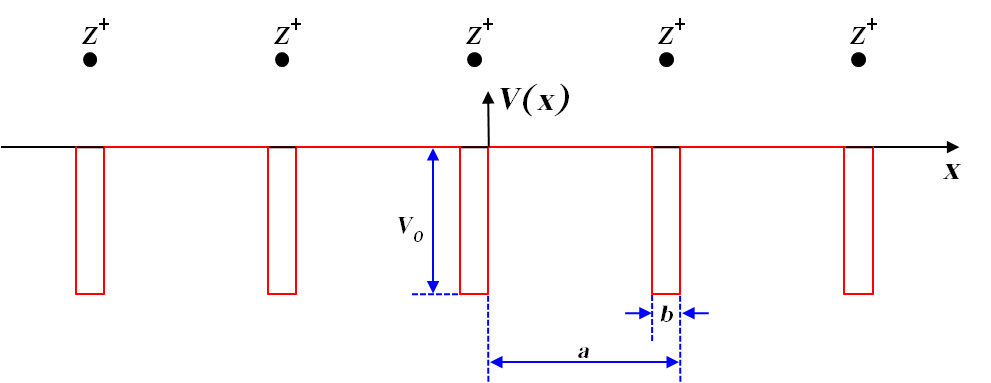
\includegraphics[width=0.75\textwidth]{Periodic_square_potential_130707} 
		\end{figure*}
		
	 	Then
		\begin{align}
			(A - \lambda I) u_{l} & = \sum_{i \in \N} \left[ (- \frac{d^{2}}{dx^{2}} - \lambda) u_{l}|_{(x_{i}, x_{i+1})} \cdot \mathds{1}_{(x_{i}, x_{i+1})} \right] \label{eq:sepofspectraleq} \\
				& = \sum_{i \in \N} \left[ \left(- \frac{d^{2}}{dx^{2}} - \lambda \right) \left( \eta\left(\frac{|\cdot|}{l}\right) \psi_{s}(\cdot, k) \right)\Big|_{(x_{i}, x_{i+1})} \cdot \mathds{1}_{(x_{i}, x_{i+1})} \right] \notag \\
				& = \sum_{i \in \N} \left[ \eta\left(\frac{|\cdot|}{l}\right) \left(- \frac{d^{2}}{dx^{2}} - \lambda \right) \psi_{s}(\cdot, k) |_{(x_{i}, x_{i+1})} \cdot \mathds{1}_{(x_{i}, x_{i+1})} \right] + R \notag
		\end{align}
		where $R$ is a sum of products of derivatives of order $\geq 1$ of $\eta\left(\frac{|\cdot|}{l}\right)$, and derivatives of order $\leq 1$ of $\psi_{s}(\cdot, k)$. Thus, note that $\psi_{s}(\cdot, k) \in H^{2}_{loc}(\R)$, the semi-periodic structure of $\psi_{s}(\cdot, k)$ implies
		\begin{equation}
			 \| R \|_{L^{2}(\R)} \leq \frac{c}{l} \| \psi_{s}(\cdot, k) \|_{H^{1}((\frac{l}{2}, \frac{l}{2}))} \leq c \frac{1}{\sqrt{l}}. \label{eq:estimofR}
		\end{equation}
		Together with \eqref{UIclosed}, \eqref{firstinclusion-firstequation} and \eqref{eq:sepofspectraleq}, this gives
		\[ \frac{1}{\|u_{l}\|}\| (A - \lambda I) u_{l} \| \leq \frac{c}{l} \]
		Now, as moreover $u_{l} \in \mathcal{D}(A)$ this results in
			\[ \frac{1}{\|u_{l} \|} \| (A - \lambda I) u_{l} \| \rightarrow 0 \text{ as } l \rightarrow \infty \]
		Thus, either $\lambda$ is an eigenvalue of $A$, or $(A - \lambda I)^{-1}$ exists but is unbounded. In both cases, $\lambda \in \sigma(A)$.
	\end{proof}
\end{theorem}	

The other inclusion can be shown by using the previous shown properties of the Floquet transformation and the completeness of the Bloch waves. Hence, this prove doesn't differ from the one for an arbitrary m-th order linear differential operator with periodic coefficients. Again, due to completeness I still want to list the proof here, even though one can find it for example in \cite[Chap. 3]{Plum10}

\begin{theorem} \label{4.1:thm-MainResult.SecondInclusion}

	$\sigma(A) \subset \bigcup_{s \in \N} I_{s}.$

	\begin{proof}
		Let $\lambda \in \R \setminus \bigcup_{s \in \N} I_{s}$. Hence, due to \eqref{UIclosed}, there exists some $\delta > 0$ such that
			\begin{equation}
				|\lambda_{s}(k) - \lambda| \geq \delta \quad \text{ for all } s \in \N, k \in B \label{lambda-distance}
			\end{equation} We have to prove that $\lambda \in \rho(A)$, i.e. for each $f \in L^{2}(\R)$ there exists some $u \in \mathcal{D}(A)$ satisfying $(A-\lambda I)u = f$. For an arbitrary $f \in L^{2}(\R)$ and $l \in \N$, we define 
			\[ f_{l}(x) \coloneqq \frac{1}{\sqrt{|B|}} \sum_{s=1}^{l} \int_{B} \langle (Uf)(\cdot, k), \psi_{s}(\cdot, k)\rangle_{L^{2}(\Omega)} \psi_{s}(x,k) dk \]
			and
			\begin{equation}
				u_{l} \coloneqq \frac{1}{\sqrt{|B|}} \sum_{s=1}^{l} \int_{B} \frac{1}{\lambda_{s}(k) - \lambda} \langle (Uf)(\cdot, k), \psi_{s}(\cdot, k)\rangle_{L^{2}(\Omega)} \psi_{s}(x, k) dk \label{ul}
			\end{equation} 

		As $\lambda$ is chosen to be outside of the spectrum the operator $A_{k} - \lambda I$ is invertible, therefore the following equation has for every $f \in L^{2}(\R)$ and $k \in \overline{B}$ a unique solution $v \in \mathcal{D}(A_{k})$
		\begin{equation}
			(A_{k} - \lambda I) v(\cdot, k) = (Uf)(\cdot, k) \quad \text{ on } \Omega. \label{4.9}			
		\end{equation}
		Due to \eqref{4.9}, both $v(\cdot, k)$ and $\psi_{s}(\cdot, k)$ satisfy semi-periodic boundary conditions. Hence, \eqref{eigv-problem}, \eqref{lambda-distance} and Parseval's identity yield
		\begin{align*}
			\| (Uf)(\cdot, k)\|^{2}_{L^{2}(\Omega)} & = \sum_{s=1}^{\infty} |\langle (Uf)(\cdot, k), \psi_{s}(\cdot, k)\rangle_{L^{2}(\Omega)}|^{2} \\ % todo prove this
			& = \sum_{s=1}^{\infty}|\langle (A_{k} - \lambda) v(\cdot, k), \psi_{s}(\cdot, k)\rangle_{L^{2}(\Omega)}|^{2} \\
			& = \sum_{s=1}^{\infty} |\lambda_{s}(k) - \lambda|^{2} |\langle v(\cdot, k), \psi_{s}(\cdot, k)\rangle_{L^{2}(\Omega)}|^{2} \\
			& \geq \delta^{2} \| v(\cdot, k)\|^{2}_{L^{2}(\Omega)}.
		\end{align*}
		By Theorem \ref{3.2:thm-UIsometricIsomorphism} we know that $f \in L^{2}(\Omega \times B)$, this implies $v \in L^{2}(\Omega \times B)$, and we can define $u \coloneqq U^{-1} v \in L^{2}(\R)$. Thus, \eqref{4.9} gives
			\begin{align*}
				\langle (Uf)(\cdot, k), \psi_{s}(\cdot, k) \rangle_{L^{2}(\Omega)} & = \langle (A_{k} - \lambda I)(Uu)(\cdot, k), \psi_{s}(\cdot, k) \rangle_{L^{2}(\Omega)} \\
					& = \langle (Uu)(\cdot,k), (A_{k} - \lambda I) \psi_{s}(\cdot, k) \rangle_{L^{2}(\Omega)} \\
					& = (\lambda_{s}(k) - \lambda) \langle Uu(\cdot, k), \psi_{s}(\cdot, k) \rangle_{L^{2}(\Omega)}.
			\end{align*}
		Now, we are able to apply Theorem \ref{3.3:thm-flConvergence} this yields for \eqref{ul} that
			\[ u_{l}(x) = \frac{1}{\sqrt{|B|}} \sum_{s=1}^{l} \int_{B} \langle (Uu)(\cdot, k), \psi_{s}(\cdot, k)\rangle_{L^{2}(\Omega)} \psi_{s}(x, k) dk, \]
		and whence Theorem \ref{3.3:thm-flConvergence} gives
			\begin{equation}
				u_{l} \rightarrow u, \quad f_{l} \rightarrow f \quad \text{ in } L^{2}(\R) \text{ as } l \rightarrow \infty. \label{ulflconvergence}
			\end{equation}
		We will now prove that
		\begin{equation}
				\langle u_{l}, (A - \lambda I) v \rangle = \langle f_{l}, v\rangle \text{ for all } l \in \N, v \in \mathcal{D}(A); \label{lefttoprove}
			\end{equation} 
		As $A$ is self-adjoint, by Theorem \ref{2.3:thm-ASelfAdjoint}, this implies $u_{l} \in \mathcal{D}(A)$, and $(A - \lambda I) u_{l} = f_{l}$ for all $l \in \N$. As furthermore every self-adjoint operator is also closed, \eqref{ulflconvergence} now implies
			\[ u \in \mathcal{D}(A) \text{ and } (A - \lambda I) u = f, \]
		which is the desired result.
		~\newline ~\newline
		Eventually, we are left to prove \eqref{lefttoprove}. So, let $\varphi \in C_{0}^{\infty}(\R)$ be fixed, and let $K \subseteq \R$ denote an open interval containing $\supp(\varphi)$ in its interior. By Fubini's Theorem we know that 
		\begin{align*}
			r_{s}(x, k) & \coloneqq \frac{1}{\lambda_{s}(k) - \lambda} \langle (Uf)(\cdot, k), \psi_{s}(\cdot, k) \rangle_{L^{2}(\Omega)} \psi_{s}(x, k) \overline{(A - \lambda I) \varphi(x)}, 
			\intertext{and}
			t_{s}(x, k) & \coloneqq \langle (Uf)(\cdot, k), \psi_{s}(\cdot, k) \rangle_{L^{2}(\Omega)} \psi_{s}(x, k) \overline{\varphi(x)}
		\end{align*}
		are in $L^{2}(K \times B)$, since \eqref{lambda-distance}, $(A_{k} - \lambda I) \varphi \in L^{\infty}(K)$ and $\varphi \in L^{\infty}(K)$ imply 
		\[ \| r_{s} \|_{L^{2}(K \times B)} \leq c \| (Uf)(\cdot, k) \|^{2}_{L^{2}(\Omega)} \| \psi_{s}(\cdot, k) \|^{2}_{L^{2}(K)}
		\]
		and analogously for $t_{s}$.	 Now	, as $K$ is bounded there exists a finite number of copies of $\Omega$ such that they cover $K$, hence $\psi_{s}(\cdot, k)$ is in $L^{2}(K)$ as a function of $k$, and $(Uf)(\cdot, k)$ is in $L^{1}(B)$ by Theorem \ref{3.2:thm-UIsometricIsomorphism}. Since $B$ is equally bounded, $r$ and $t$ are also in $L^{1}(K \times B)$. Therefore, Fubini’s Theorem implies that the order of integration with respect to $x$ and $l$ may be exchanged for $r$ and $t$. Thus, by \eqref{ul}, the fact that $\varphi$ has compact support in the interior of $K$ and \eqref{eigv-problem} we conclude
			\begin{align*}
				\int_{K} u_{l}(x) \overline{(A - \lambda I) \varphi(x)} dx & = \frac{1}{\sqrt{|B|}} \sum_{s=1}^{l} \int_{K} \left( \int_{B} r_{s}(x, k) dk \right) dx \\
					& = \frac{1}{\sqrt{|B|}} \sum_{s=1}^{l} \int_{B} \langle (Uf)(\cdot, k), \psi_{s}(\cdot, k) \rangle_{L^{2}(\Omega)} \langle \psi_{s}(\cdot, k), \varphi \rangle_{L^{2}(K)} dk \\
					& = \int_{K} \left[ \frac{1}{\sqrt{|B|}} \sum_{s=1}^{l} \int_{B} \langle (Uf)(\cdot, k), \psi_{s}(\cdot, k) \rangle_{L^{2}(\Omega)} \psi_{s}(x, k) dk \right] \overline{\varphi(x)} dx \\
					& = \int_{K} f_{l}(x) \overline{\varphi(x)} dx,
			\end{align*}
			i.e. \eqref{lefttoprove}.
	\end{proof}
\end{theorem}